\definecolor{c06p1blue}{HTML}{2A78D6}
\definecolor{c06p1orange}{HTML}{EB6834}
\definecolor{c06p1gray}{HTML}{52514E}

\section{Demand in characteristic space}\label{sec:06-charspace}

\subsection{Products as bundles of characteristics}\label{sec:06-bundles}

The demand systems of \cref{ch:aids} are written in product space. Each good carries its own parameters,
and the model states directly how the demand for one good responds to the price of another. This chapter
develops the alternative. In the \emph{characteristics approach}, a product is a bundle of characteristics,
and consumers have preferences over the characteristics rather than over the products themselves
\citep{Lancaster1966,Gorman1980}. A car is a combination of size, engine power, fuel economy and brand. A
breakfast cereal is a combination of sugar, fiber, texture and taste. Two products are close substitutes when
they offer similar characteristics at similar prices.

The empirical form of the approach is a \emph{discrete choice} model \citep{McFadden1974}. Each consumer buys
at most one unit of one product, or buys nothing. Consumers differ in their tastes, so they choose different
products, and in the aggregate every product is chosen by someone. The market demand for a product is the
mass of consumers for whom that product is the best option. Aggregate demand therefore depends on the entire
distribution of consumer tastes. A single representative taste cannot summarize it, because the products that
compete for the marginal consumers determine the substitution patterns.

\subsection{Product space and characteristic space}\label{sec:06-ps-cs}

The first advantage of the characteristics approach is dimensionality. Consider a linear demand system
$q = a + Ap$ for $J$ products, where $q$ and $p$ are $J$-vectors. The $J\times J$ matrix $A$ contains $J^2$
price coefficients. With $J = 50$ brands the system has \num{2500} price coefficients, and a log-linear system
has the same count \citep[footnote 1]{BerryPakes2007}.\footnote{Throughout the chapter, page, footnote, equation
and table numbers of \citet{BerryPakes2007} refer to the author manuscript dated July 2, 2007 (41 pages). They do
not refer to the pagination of the article in the \emph{International Economic Review} 48(4), 1193--1225.} The
restrictions of consumer theory and the separability
assumptions of \cref{ch:aids} reduce this number, but the count still grows with $J$. In a characteristics
model the number of parameters grows with the number $K$ of characteristics and with the dimension of consumer
heterogeneity. A model in which each of $K$ characteristics has a mean taste and a standard deviation of tastes
has $2K$ taste parameters, whatever the number of products.

The second advantage concerns new products. A product that is a new combination of existing characteristics
can be placed in the estimated demand system before it is launched. A new car whose size and engine power lie
inside the range of existing models is an example. Products with new characteristics are a different matter.
The first electric cars offered a driving range, a charging time and an absence of fuel costs that no existing
car had. The data on existing cars contain no information on how consumers value those characteristics, so the
model cannot predict their demand.

The characteristics approach has several drawbacks.
\begin{enumerate}
  \item It needs more data. The researcher must observe the relevant characteristics of every product, and
  the richer models also use information on consumers.
  \item Estimation is harder. Market shares are integrals over the distribution of tastes, so estimation
  involves nonlinear optimization and often simulation.
  \item The functional forms can have restrictive or odd implications. The leading example is the ``too many
  characteristics'' problem of logit-type models, studied in \cref{sec:06-epsilon}.
  \item Single-choice models cannot generate complementarity. \Cref{cor:06-wdz} shows that any two goods in a
  single-choice additive random utility model are substitutes.
  \item Some attributes cannot be measured. The relevant attributes of books, films or recipes are hard to code
  as a short vector of characteristics.
\end{enumerate}
The last point underlies the objection of \citet[sec.~5.5]{Hausman1997}. He describes each brand of cereal by
its own indicator variable, because ``no reasonable metric exists to describe `how close' attributes are'' for
products such as Apple-Cinnamon Cheerios. \Cref{ch:newgoods} returns to this debate.

\subsection{Two branches of theory}\label{sec:06-branches}

The theory of competition in characteristic space has two branches. The first takes the set of products as
given and studies price competition. Its central question is the existence of a price equilibrium. The
general answer is due to \citet{CaplinNalebuff1991}.\footnote{The copy we use is Cowles Foundation Discussion Paper
937 of February 1990, the working-paper version of the article. Page numbers refer to that version.} They obtain a
pure-strategy Bertrand-Nash price equilibrium for any number of single-product firms and any configuration of
products (their Theorem~2, p.~14). Two assumptions deliver it. Their assumption A1 requires each consumer's utility
to be linear in an $n$-dimensional vector $a$ of consumer characteristics (p.~4). It is enough that A1 and the
next assumption hold for some parameterization of preferences (p.~6).

Their assumption A2 requires the density $f$ of consumer types $a$ to be \emph{$\rho$-concave} with
$\rho = -\frac{1}{n+1}$ (p.~5). A density $f$ is $\rho$-concave if $f^\rho$ is concave when $\rho > 0$, $\ln f$ is
concave when $\rho = 0$, and $f^\rho$ is convex when $\rho < 0$. A $\rho$-concave function is also $\rho'$-concave for
every $\rho' < \rho$. Log-concavity is the case $\rho = 0$, so every log-concave density satisfies A2, and A2 is the
weaker condition. It also covers the multivariate $t$ distribution with at least one degree of freedom, which
includes the multivariate Cauchy. Caplin and Nalebuff list the lognormal as a distribution that A2 excludes
(p.~6). The exclusion applies to dispersed lognormals.\footnote{With one taste dimension, $n = 1$ and A2 requires
$f^{-\frac{1}{2}}$ to be convex. Let $\ln a \sim N(0, \sigma^2)$ and $y = \ln a$. Then
$f(a)^{\rho} = C\exp(\phi(y))$ with $\phi(y) = -\rho y - \frac{\rho y^2}{2\sigma^2}$ and a constant $C > 0$. Two
applications of the chain rule give
$\frac{d^2}{da^2}f^{\rho} = \frac{f^{\rho}}{a^2}\big[\phi'(y)^2 - \phi'(y) + \phi''(y)\big]$. The term
$\phi'^2 - \phi'$ reaches its minimum $-\frac{1}{4}$ at $\phi' = \frac{1}{2}$, and $\phi'$ takes every real value.
With $\phi'' = -\frac{\rho}{\sigma^2}$ and $\rho = -\frac{1}{2}$, the density meets A2 if and only if
$\frac{1}{2\sigma^2} \ge \frac{1}{4}$, that is, $\sigma^2 \le 2$.} The proof aggregates individual demands with
theorems of Pr\'ekopa and Borell. Under A1 and A2 the reciprocal $\frac{1}{D(p)}$ of each firm's demand is convex in
its own price, so profit is quasi-concave in own price (their Proposition~4, p.~14). Kakutani's fixed point theorem
then delivers the equilibrium. They also give conditions for uniqueness. The framework covers location models,
characteristics models and probabilistic choice models such as the logit. \Cref{ch:diffprod} states and uses these
results.

The second branch lets firms choose their positions in characteristic space, with or without a later stage of
price competition. \citet{Hotelling1929} placed firms on a line and \citet{Salop1979} on a circle.
\citet{DAspremontGabszewiczThisse1979} showed that firms in Hotelling's model differentiate as much as they can
when they anticipate price competition. \citet{ShakedSutton1982} found the same force in quality choice.
\Cref{sec:06-hotelling,sec:06-vdef} state these results. The empirical literature is almost entirely about the
first branch. Empirical models of product choice are
rarer, and that gap matters for identification, as the next subsection explains.

\subsection{Endogenous characteristics and instruments}\label{sec:06-charinst}

Empirical demand models in characteristic space lead to an estimating equation of the form
\begin{equation}\label{eq:06-delta}
\delta_{jt} = x_{jt}\beta - \alpha p_{jt} + \xi_{jt}.
\end{equation}
Here $\delta_{jt}$ is the mean utility of product $j$ in market $t$. The row vector $x_{jt}$ collects its $K$
observed characteristics. The price is $p_{jt}$, and $\xi_{jt}$ is product quality that consumers and firms
observe but the econometrician does not. \Cref{sec:06-inversion-idea} explains how $\delta_{jt}$ is recovered from market
shares. Firms set prices knowing $\xi_{jt}$, so price is correlated with the error, and \cref{eq:06-delta}
must be estimated with instruments (\cref{ch:logit}).

Two families of instruments dominate. The first consists of cost shifters, variables that move marginal cost
but not utility. The second consists of functions of the characteristics of other products, such as the sums
$\sum_{k \in \mathcal{J}_f, k \neq j} x_{kt}$ and $\sum_{k \notin \mathcal{J}_f} x_{kt}$ over the firm's other
products and over rivals' products \citep{BerryLevinsohnPakes1995}. These functions shift the markup of
product $j$, because they measure how crowded its neighborhood is. When firms set prices by the multi-product
first-order condition, the effect of other products' characteristics on the price of $j$ also depends on who owns
those products. \citet[p.~29]{AckerbergEtAl2007} trace this reasoning back at least to \citet{Bresnahan1987}. He
stressed that markups are lower in ``crowded'' parts of the product space, and higher when ``nearby'' products have
the same owner.\footnote{Page numbers of \citet{AckerbergEtAl2007} refer to the author manuscript of June 14, 2006,
prepared for the \emph{Handbook of Econometrics}.} \Cref{sec:06-bresnahan} shows both effects at work in his model.
The validity of these instruments rests on the mean independence condition
\begin{equation}\label{eq:06-meanind}
\E\left[\xi_{jt} \,\middle|\, x_{1t}, \dots, x_{J_t t}\right] = 0 .
\end{equation}
Characteristics-based instruments are inefficient, and they are probably inconsistent. Most researchers know
this and use them for lack of better alternatives. The two problems are distinct.

The first problem is consistency. Condition \eqref{eq:06-meanind} treats characteristics as exogenous. Firms
choose characteristics, however, and they know $\xi_{jt}$ when they design products. The design team even has
some control over $\xi_{jt}$ itself \citep[p.~30]{AckerbergEtAl2007}. A carmaker that knows its
new model has an attractive design may also give it a larger engine. Rivals may position their products close
to a successful product. In both cases $x_{jt}$ is correlated with $\xi_{jt}$, the moment condition fails, and
the instrumental variables estimator is inconsistent. Predetermination does not repair the problem. A
characteristic chosen before prices does not respond to shocks realized at the pricing stage. It still
responds to any component of $\xi_{jt}$ that the firm could foresee at the design stage. Condition
\eqref{eq:06-meanind} needs a timing and information assumption: the firm fixes $x_{jt}$ before it learns
$\xi_{jt}$, and $\xi_{jt}$ is unpredictable at that time. This is where the second branch of theory meets
identification. If product positioning is endogenous, characteristics cannot serve as instruments without a
model of how they were chosen.

The second problem is efficiency. Suppose \eqref{eq:06-meanind} holds. Then every function of the
characteristics is a valid instrument, and sums of rival characteristics are an arbitrary choice.
\citet{Chamberlain1987} derives the efficient instrument for a conditional moment restriction
$\E[\xi_{jt}(\theta_0) \mid z_t] = 0$, where $z_t$ collects the exogenous variables of market $t$. Under
conditional homoskedasticity it is proportional to
\begin{equation}\label{eq:06-optiv}
D(z_t) = \E\left[\frac{\partial \xi_{jt}(\theta_0)}{\partial \theta} \,\middle|\, z_t\right].
\end{equation}
Ad hoc sums of characteristics do not reproduce this function. In addition, characteristics vary little
across markets and over time, so instruments built from them are often weak. \Cref{ch:blp} discusses
approximations to \eqref{eq:06-optiv}.

We now make the characteristics approach precise. \Cref{sec:06-rum} writes it as a random utility model and
aggregates individual choices into market shares. \Cref{sec:06-tiev} derives the closed forms that one
distribution of the idiosyncratic shock delivers. These two sections supply the language in which every
demand model of this chapter and of \cref{ch:logit,ch:blp} is written.

\section{Random utility and aggregation to market shares}\label{sec:06-rum}

\subsection{The random utility model}\label{sec:06-rum-setup}

We consider a market with consumers $i = 1, \dots, I$ and products $j = 0, 1, \dots, J$. Product $0$ is the
\emph{outside good}, the option of buying none of the inside products $\mathcal{J} = \{1, \dots, J\}$. We
suppress the market index $t$ when no confusion arises. Consumer $i$ obtains utility
\begin{equation}\label{eq:06-utility}
u_{ij} = U(x_j, p_j, \xi_j, \nu_i; \theta), \qquad j = 0, 1, \dots, J,
\end{equation}
from product $j$. Here $\nu_i$ is a vector of consumer tastes drawn from a distribution $F$, and $\theta$ is a
vector of demand parameters. The conduct parameter of \cref{ch:conduct} does not appear in this chapter. Firm
conduct enters through the ownership or cooperation matrix $\Omega$ instead (\cref{sec:06-bresnahan}). The
consumer buys product $j$ if and only if $u_{ij} \ge u_{ik}$ for every $k$.

\begin{definition}[Random utility model and market shares]\label{def:06-rum}
A \emph{random utility model} specifies the utility function \eqref{eq:06-utility} and the taste distribution
$F$. The \emph{acceptance set} of product $j$ is the set of tastes for which $j$ is optimal,
\begin{equation}\label{eq:06-acceptance}
A_j(\theta) = \left\{\nu : U(x_j, p_j, \xi_j, \nu; \theta) \ge U(x_k, p_k, \xi_k, \nu; \theta)
\text{ for all } k = 0, 1, \dots, J\right\}.
\end{equation}
The \emph{market share} of product $j$ is the probability mass of its acceptance set,
\begin{equation}\label{eq:06-share}
s_j(\theta) = \int \indic\{\nu \in A_j(\theta)\}\,\dd F(\nu) = \Pr\big(\nu_i \in A_j(\theta)\big).
\end{equation}
With $M$ potential buyers in the market, the demand for product $j$ is $q_j = M s_j(\theta)$.
\end{definition}

The acceptance sets of two products can overlap only at tastes where the consumer is indifferent between them.
We rule out such ties with positive probability.

\begin{assumption}[No ties]\label{ass:06-noties}
For every pair $j \neq k$,
$\Pr\big(U(x_j, p_j, \xi_j, \nu_i; \theta) = U(x_k, p_k, \xi_k, \nu_i; \theta)\big) = 0$.
\end{assumption}

The assumption holds in the models of this book. In an additive model $u_{ij} = V_{ij} + \epsilon_{ij}$ with a
continuously distributed vector $\epsilon_i$, a tie requires $\epsilon_{ij} - \epsilon_{ik} = V_{ik} - V_{ij}$,
an event of probability zero. In the vertical model of \cref{sec:06-vertical}, two products tie for a single
value of the scalar taste, which has probability zero when $F$ is continuous. Under \cref{ass:06-noties} the
acceptance sets partition the taste space up to a null set, and
\begin{equation*}
\sum_{j=0}^{J} s_j(\theta) = 1 .
\end{equation*}
The market size $M$ counts the potential buyers, including those who choose the outside good. It is never
observed directly. The researcher must assume it, for example as the number of households in a market, and
the choice affects the estimates through the outside share $s_0 = 1 - \sum_{j \ge 1}\frac{q_j}{M}$.

\casehead{The latent variable formulation}
\citet[sec.~3.1]{McFadden1984} places the random utility model inside a broader class of qualitative response
models. Let $m$ responses be indexed by $j = 1, \dots, m$. A vector of latent variables
$y^* = x\beta - \epsilon$ takes values in $\R^h$, and $\epsilon$ has distribution $F(\epsilon \mid x)$. A
partition $A_1, \dots, A_m$ of $\R^h$ defines a generalized indicator: response $j$ is observed if and only if
$y^* \in A_j$. The response probability is
\begin{equation}\label{eq:06-latent}
P_j = \Pr(x\beta - \epsilon \in A_j \mid x) = F\big(\{x\beta\} - A_j \mid x\big),
\qquad \{x\beta\} - A_j = \{\epsilon : x\beta - \epsilon \in A_j\}
\end{equation}
\citep[eq.~3.2, p.~1403]{McFadden1984}. Utility maximization is the case $h = m$ in which $y_j^*$ is the
utility of alternative $j$ and $A_j$ is the set of latent vectors whose $j$-th component is largest. The same
apparatus covers ordered responses, where a scalar latent variable falls between thresholds, and vectors of
binary responses, where the sets $A_j$ are products of half-lines \citep[pp.~1403--1404]{McFadden1984}.

Two observations of \citet{McFadden1984} frame the rest of this chapter. The first concerns the meaning of
the disturbance. It may represent factors known to the decision maker but not to the econometrician. It may
also represent randomness in the decision protocol itself, so that the same person facing the same options
could choose differently. \citet[p.~1412]{McFadden1984} notes that the two readings cannot ordinarily be
distinguished, unless the decision protocol is observable or individuals face many decisions in experiments.
The second concerns the direction of modeling. One could write down a convenient probability model and then
ask whether a population of utility maximizers could have generated it. For consumers, the known sufficient
conditions for this are quite restrictive \citep[p.~1406]{McFadden1984}. The additive random utility models
of \cref{sec:06-arum} avoid the question by construction: they start from utilities and derive the
probabilities.

\casehead{What the shock represents}
In applications the idiosyncratic term has several readings. It may capture consumer characteristics that the
econometrician does not observe, such as the distance from a consumer's home to a dealer. It may capture
product characteristics that consumers value differently. It may absorb measurement error in prices or
characteristics, or the approximation error of a parametric utility function. Finally, it may reflect
psychological biases or optimization errors. The last reading matters for welfare. The welfare formulas of
\cref{sec:06-logsum} count the realized shock as utility. If the shock is a mistake, those formulas overstate
the benefit of choice, a point taken up in \cref{sec:06-epsilon} and \cref{ch:newgoods}.

\casehead{Why a structural error is needed}
The product-level term $\xi_j$ plays the role of the error in a classical demand and supply model. Without it,
a model with a few parameters cannot fit $J$ observed shares, because products with identical observed
characteristics would have identical predicted shares. With it, the model fits the data, and the source of
price endogeneity becomes explicit: firms see $\xi_j$ when they set prices. \Cref{ch:logit} treats the
resulting instrumental variables problem in full.

\casehead{Single-unit purchases}
The model assumes that each consumer buys one unit of one product. This is a good approximation for durable
goods bought one at a time, such as cars, airline tickets and houses. It is a poor approximation for groceries.
A household buys several units and several varieties of cereal or yogurt on a single trip, so a single-choice
model misses both the quantity decision and any complementarity between varieties. Extensions handle
multiple discrete choices \citep{Hendel1999}, treated in \cref{ch:logit}, and bundles of complementary goods
\citep{Gentzkow2007}, treated in \cref{ch:newgoods}.

\subsection{The outside good}\label{sec:06-outside}

Most demand models in characteristic space include an outside good. Three reasons favor it, and one cost
comes with it.
\begin{enumerate}
  \item It allows the demand for the whole category to respond to prices. Without it, a common price increase
  leaves total category demand unchanged (\cref{prop:06-outside}).
  \item It provides the location normalization of utility. Inside utilities are measured relative to the
  utility of not buying (\cref{prop:06-normalization}).
  \item It is needed for welfare analysis. A new product can draw consumers who previously bought nothing,
  and its value depends on how many do.
  \item It has a cost. Shares of the outside good require a definition of market size, which is an
  assumption.
\end{enumerate}

\begin{proposition}[Demand without an outside good]\label{prop:06-outside}
Suppose consumers choose only among the inside products $j = 1, \dots, J$, with
\begin{equation*}
u_{ij} = x_j\beta + \xi_j - \alpha_i p_j + \mu_{ij} + \epsilon_{ij},
\end{equation*}
where $\alpha_i > 0$, and $\mu_{ij}$ and $\epsilon_{ij}$ do not depend on prices. For every scalar $c$ and
every product $j$, $s_j(p + c\mathbf{1}) = s_j(p)$, where $\mathbf{1}$ is the $J$-vector of ones. Hence total
category demand equals $M$ at all prices. Moreover, consider a firm that owns all $J$ products and has constant
marginal costs $mc_j$. Its profit satisfies $\Pi(p + c\mathbf{1}) = \Pi(p) + cM$, which is unbounded in $c$, so
the firm has no finite profit-maximizing price vector.
\end{proposition}

\begin{proof}
Raising every price by $c$ changes each utility of consumer $i$ by the same amount:
\begin{equation*}
u_{ij}(p + c\mathbf{1}) = u_{ij}(p) - \alpha_i c \qquad \text{for all } j.
\end{equation*}
The utility differences $u_{ij} - u_{ik}$ are unchanged, so every consumer makes the same choice and every share
is unchanged. Total demand is $M\sum_{j=1}^J s_j = M$. For the profit of the multi-product firm,
\begin{align*}
\Pi(p + c\mathbf{1}) &= \sum_{j=1}^J (p_j + c - mc_j)\,M s_j(p + c\mathbf{1}) \\
&= \sum_{j=1}^J (p_j - mc_j)\,M s_j(p) + cM\sum_{j=1}^J s_j(p) \\
&= \Pi(p) + cM .
\end{align*}
The last expression grows without bound as $c \to \infty$.
\end{proof}

The result depends on two features: the absence of an outside option and utility that is linear in price.
With an outside good $u_{i0} = \epsilon_{i0}$ whose price is normalized to zero, a common price increase lowers
every inside utility relative to the outside option, and the inside shares fall. With income effects, a
common price increase changes utility differences, because the marginal utility of money changes with the
money left over. The outside good is the natural fix, and every discrete choice model in the rest of the book includes one.

\subsection{Normalizations and what is identified}\label{sec:06-normalization}

Utility is ordinal. Only the ranking of alternatives matters for choice, so many utility functions generate the
same choices. The next proposition states the invariance that drives the normalizations used in practice.

\begin{proposition}[Invariance of choices]\label{prop:06-normalization}
Let $\tilde u_{ij} = a_i + b_i u_{ij}$ for $j = 0, 1, \dots, J$, where $a_i$ and $b_i > 0$ may depend on the
consumer, on her tastes and on anything common to all alternatives, but not on $j$. Then consumer $i$ makes the
same choice under $\tilde u$ as under $u$, and every acceptance set and every market share is unchanged.
\end{proposition}

\begin{proof}
For any pair $j, k$,
\begin{equation*}
\tilde u_{ij} \ge \tilde u_{ik}
\iff a_i + b_i u_{ij} \ge a_i + b_i u_{ik}
\iff u_{ij} \ge u_{ik},
\end{equation*}
where the last step divides by $b_i > 0$. The optimal choice is therefore the same for every taste vector. The
acceptance sets \eqref{eq:06-acceptance} and the shares \eqref{eq:06-share} are unchanged.
\end{proof}

The same argument applies to any strictly increasing transformation that is common to the alternatives. Two
normalizations follow.
\begin{enumerate}
  \item \emph{Location.} Setting $a_i = -u_{i0}$ and $b_i = 1$ gives $\tilde u_{i0} = 0$. Inside utilities are
  then measured relative to the outside good. When the outside utility contains a random term,
  $u_{i0} = V_{i0} + \epsilon_{i0}$, the usual normalization sets only its deterministic part to zero,
  $V_{i0} = 0$.
  \item \emph{Scale.} Setting $b_i = \frac{1}{\sigma_\epsilon}$ in a model $u_{ij} = V_{ij} + \sigma_\epsilon
  \epsilon_{ij}$ removes the scale of the shock. The parameter vectors $(\beta, \alpha, \sigma_\epsilon)$ and
  $(c\beta, c\alpha, c\sigma_\epsilon)$ with $c > 0$ are observationally equivalent. We must fix one of them,
  either the variance of the shock or one coefficient. In the vertical model of \cref{sec:06-vertical} the
  analogous step fixes the mean of the price sensitivity $\nu_i$.
\end{enumerate}
A consumer-specific scale $b_i$ is also not identified separately from tastes. A model in which the scale of
utility varies across consumers is observationally equivalent to a random coefficients model in which all of a
consumer's coefficients move in proportion.

\begin{remark}[Variables that do not vary across alternatives]\label{rem:06-invariant}
A consumer attribute that enters all utilities in the same way cancels from every comparison. In
$u_{ij} = x_j\beta + z_i\gamma + \epsilon_{ij}$, the term $z_i\gamma$ drops out, and $\gamma$ is not identified
from choices \citep[p.~1412]{McFadden1984}. Consumer attributes matter only through interactions with
alternative-specific terms. Examples are an income-price interaction, or the specification
$z_i\gamma_j$ with alternative-specific coefficients. The latter needs a normalization such as $\gamma_0 = 0$
\citep[eq.~3.16, p.~1413]{McFadden1984}. The same logic restricts the multinomial probit of
\cref{sec:06-probit}. Only the covariance matrix of utility differences matters, and it is identified only up to
scale. With $J+1$ alternatives the differences relative to one alternative have a $J\times J$ covariance matrix
with $\frac{J(J+1)}{2}$ distinct elements, and one of them is fixed by the scale normalization.
\end{remark}

\casehead{Income}
Income enters utility through a function $f(y_i, p_j)$ of income $y_i$ and price,
\begin{equation}\label{eq:06-income}
u_{ij} = f(y_i, p_j) + \delta_j + \mu_{ij} + \epsilon_{ij}.
\end{equation}
In this subsection $\delta_j$ collects only the non-price part of mean utility, because price enters through $f$.
Economic sense suggests $f_y > 0$, $f_p < 0$ and $f_{py} \ge 0$. The first says that money left over raises
utility. The second says that price lowers it. The third says that the marginal disutility of price falls with
income, so richer consumers are less price sensitive. \Citet{BerryLevinsohnPakes1995} use
$f(y_i, p_j) = \alpha\ln(y_i - p_j)$, for which
\begin{align*}
f_y &= \frac{\alpha}{y_i - p_j} > 0, \\
f_p &= -\frac{\alpha}{y_i - p_j} < 0, \\
f_{py} &= \frac{\partial}{\partial y_i}\left(-\frac{\alpha}{y_i - p_j}\right) = \frac{\alpha}{(y_i - p_j)^2} > 0 .
\end{align*}
The price sensitivity $-f_p$ falls as income rises. The quasi-linear form $f(y_i, p_j) = \alpha(y_i - p_j)$
has $f_{py} = 0$. The term $\alpha y_i$ is then common to all alternatives, including the outside good with
$u_{i0} = \alpha y_i + \epsilon_{i0}$, and it cancels by \cref{prop:06-normalization}. Income matters for
choices only when $f_{py} \neq 0$ or when income interacts with other terms.

\subsection{Additive random utility and the social surplus function}\label{sec:06-arum}

Most empirical models separate utility into a part that depends on observables and parameters and an additive
random part.

\begin{definition}[Additive random utility model]\label{def:06-arum}
An \emph{additive random utility model} (ARUM) has
\begin{equation}\label{eq:06-arum}
u_{ij} = V_{ij} + \epsilon_{ij}, \qquad j = 0, 1, \dots, J,
\end{equation}
where $V_{ij}$ is a deterministic function of product attributes, consumer attributes and parameters. The
vector $\epsilon_i = (\epsilon_{i0}, \dots, \epsilon_{iJ})$ has a joint density, finite means, and is independent
of $V_i = (V_{i0}, \dots, V_{iJ})$. The choice probabilities are
\begin{equation*}
P_j(V_i) = \Pr\big(V_{ij} + \epsilon_{ij} > V_{ik} + \epsilon_{ik} \text{ for all } k \neq j\big).
\end{equation*}
The \emph{social surplus function} is the expected maximum utility,
\begin{equation}\label{eq:06-G}
G(V) = \E\Big[\max_{j = 0, \dots, J}\,(V_j + \epsilon_j)\Big].
\end{equation}
\end{definition}

Random coefficients fit this definition conditional on the taste draw. With
$u_{ij} = \delta_j + \mu_{ij} + \epsilon_{ij}$, we set $V_{ij} = \delta_j + \mu_{ij}$ for a given draw $\nu_i$,
and the market share averages $P_j(V_i)$ over the distribution of $\nu_i$. The next theorem is the
foundation of welfare analysis with discrete choice models.

\begin{theorem}[Williams, Daly and Zachary]\label{thm:06-wdz}
Under \cref{def:06-arum}, the social surplus function has the following properties.
\begin{enumerate}[label=(\roman*)]
  \item $G$ is finite and convex, and $G(V + c\mathbf{1}) = G(V) + c$ for every scalar $c$.
  \item $G$ is differentiable, and $\frac{\partial G(V)}{\partial V_j} = P_j(V)$ for every $j$.
\end{enumerate}
\end{theorem}

\begin{proof}
Write $m(V, \epsilon) = \max_j (V_j + \epsilon_j)$, so that $G(V) = \E[m(V, \epsilon)]$.

\emph{Finiteness.} Since $|m(V, \epsilon)| \le \sum_j |V_j| + \sum_j |\epsilon_j|$ and each $\epsilon_j$ has a finite
mean, $G(V)$ is finite.

\emph{Translation.} Adding $c$ to every $V_j$ adds $c$ to every term inside the maximum:
\begin{equation*}
m(V + c\mathbf{1}, \epsilon) = \max_j (V_j + c + \epsilon_j) = c + m(V, \epsilon).
\end{equation*}
Taking expectations gives $G(V + c\mathbf{1}) = G(V) + c$.

\emph{Convexity.} For fixed $\epsilon$, $V \mapsto m(V, \epsilon)$ is the maximum of the affine functions
$V \mapsto V_j + \epsilon_j$, so it is convex. For $\lambda \in [0,1]$,
\begin{equation*}
m(\lambda V + (1-\lambda)V', \epsilon) \le \lambda m(V, \epsilon) + (1-\lambda) m(V', \epsilon).
\end{equation*}
Taking expectations preserves the inequality, so $G$ is convex.

\emph{Derivative.} Fix $j$ and let $e_j$ be the $j$-th unit vector. Because $\epsilon$ has a density, the
event that two alternatives tie has probability zero. Fix a realization $\epsilon$ without ties. If $j$ is the
unique maximizer, then for $h$ small enough $j$ remains the maximizer, and
$m(V + he_j, \epsilon) - m(V, \epsilon) = h$. If $j$ is not the maximizer, then for $h$ small enough the
maximum does not change. Hence
\begin{equation*}
\lim_{h \to 0}\frac{m(V + he_j, \epsilon) - m(V, \epsilon)}{h} = \indic\{j \text{ maximizes } V_k + \epsilon_k\}
\end{equation*}
for almost every $\epsilon$. The maximum changes by at most $|h|$ when one argument changes by $h$, so the
difference quotient is bounded by one in absolute value. By dominated convergence,
\begin{equation*}
\frac{\partial G(V)}{\partial V_j}
= \E\left[\lim_{h\to 0}\frac{m(V + he_j, \epsilon) - m(V, \epsilon)}{h}\right]
= \Pr\big(j \text{ maximizes } V_k + \epsilon_k\big) = P_j(V).
\end{equation*}
A convex function whose partial derivatives exist at a point is differentiable at that point, which completes
the proof.
\end{proof}

The result is due to \citet{Williams1977} and \citet{DalyZachary1978}, and \citet{McFadden1981} developed it.
Its corollaries are the discrete choice counterparts of the integrability conditions of consumer theory.

\begin{corollary}[Properties of choice probabilities]\label{cor:06-wdz}
Under \cref{def:06-arum}, the following hold.
\begin{enumerate}[label=(\alph*)]
  \item $\sum_{j=0}^J P_j(V) = 1$.
  \item $P_j(V + c\mathbf{1}) = P_j(V)$, so $\sum_{k=0}^J \frac{\partial P_j}{\partial V_k} = 0$ wherever $P_j$ is
  differentiable.
  \item $\frac{\partial P_j}{\partial V_k} \le 0$ for $k \neq j$, and $\frac{\partial P_j}{\partial V_j} \ge 0$.
  \item If $G$ is twice continuously differentiable,
  $\frac{\partial P_j}{\partial V_k} = \frac{\partial P_k}{\partial V_j}$ for all $j, k$.
\end{enumerate}
\end{corollary}

\begin{proof}
For (a), differentiate the translation property of \cref{thm:06-wdz} with respect to $c$:
$\sum_j \frac{\partial G}{\partial V_j} = 1$. For (b), the event that $j$ is chosen does not change when all
$V_k$ rise by $c$. Differentiating $P_j(V + c\mathbf{1}) = P_j(V)$ with respect to $c$ gives the sum. For (c),
raising $V_k$ with $k \neq j$ shrinks the event $\{V_j + \epsilon_j > V_l + \epsilon_l \text{ for all } l \neq j\}$,
so $P_j$ weakly falls. The own derivative then satisfies
$\frac{\partial P_j}{\partial V_j} = -\sum_{k\neq j}\frac{\partial P_j}{\partial V_k} \ge 0$ by (b). For (d),
$\frac{\partial P_j}{\partial V_k} = \frac{\partial^2 G}{\partial V_k\,\partial V_j}
= \frac{\partial^2 G}{\partial V_j\,\partial V_k} = \frac{\partial P_k}{\partial V_j}$ by Young's theorem.
\end{proof}

\Cref{thm:06-wdz} plays the role of Roy's identity: choice probabilities are the gradient of a surplus function.
Part (d) of the corollary is the counterpart of Slutsky symmetry. Part (c) shows that all alternatives are
substitutes in a single-choice model: an increase in the attractiveness of $k$ can only lower the probability
of choosing $j$. Since price lowers $V_k$, this means $\frac{\partial s_j}{\partial p_k} \ge 0$ for all
$k \neq j$, which is the absence of complementarity noted in \cref{sec:06-ps-cs}. \Citet{McFadden1981} also
proves a converse. Under sign conditions on its higher mixed partial derivatives, a function with the properties
of \cref{thm:06-wdz} is the social surplus function of some ARUM. For the hierarchical models of
\cref{sec:06-gev}, \citet[p.~1425]{McFadden1984} introduces a generating function $H$ whose logarithmic
derivatives are the response probabilities. He notes that it ``can be interpreted as a measure of social
utility''.

\casehead{Welfare}
The social surplus function measures welfare in money when utility is quasi-linear. Let
\begin{equation}\label{eq:06-quasilinear}
V_{ij} = \alpha(y_i - p_j) + w_j, \qquad p_0 = 0, \quad w_0 = 0,
\end{equation}
where $w_j$ collects the non-price terms. Consider a change in the environment from $(p^0, w^0)$ to
$(p^1, w^1)$, with deterministic utilities $V^0$ and $V^1$. The change may also add or remove products. The
\emph{compensating variation} $CV(\epsilon)$ of a consumer with shock vector $\epsilon$ is the income that can
be taken from her after the change while leaving her original maximum utility intact. A negative value is a
payment to her. It solves
\begin{equation*}
\max_j\big[\alpha(y_i - CV - p^1_j) + w^1_j + \epsilon_j\big] = \max_j\big[V^0_j + \epsilon_j\big].
\end{equation*}
The left side equals $\max_j(V^1_j + \epsilon_j) - \alpha\, CV$. Solving,
\begin{equation*}
CV(\epsilon) = \frac{1}{\alpha}\Big[\max_j(V^1_j + \epsilon_j) - \max_j(V^0_j + \epsilon_j)\Big].
\end{equation*}
Taking expectations over $\epsilon$ gives the expected compensating variation of \citet{SmallRosen1981},
\begin{equation}\label{eq:06-smallrosen}
\E[CV] = \frac{1}{\alpha}\big[G(V^1) - G(V^0)\big].
\end{equation}
Expected consumer surplus is therefore $\frac{G(V)}{\alpha}$ up to an additive constant. By
\cref{thm:06-wdz} its derivative with respect to a price is
$\frac{1}{\alpha}\frac{\partial G}{\partial V_k}\frac{\partial V_k}{\partial p_k} = -P_k$, the expected demand for
$k$. A price change thus has the familiar welfare cost of the area to the left of the demand curve. Without
quasi-linearity the marginal utility of money varies with income, and the welfare change has no closed form.
\Cref{sec:06-logsum} evaluates \eqref{eq:06-smallrosen} in closed form for the logit.

\subsection{A first example: two goods with additive shocks}\label{sec:06-twogoods}

The geometry of acceptance sets is easiest to see with two inside goods. Let
\begin{equation*}
u_{i0} = 0, \qquad u_{ij} = \delta_j + \epsilon_{ij}, \quad j = 1, 2,
\end{equation*}
where $(\epsilon_{i1}, \epsilon_{i2})$ has a joint density $g$. The consumer compares three utilities, and the
$(\epsilon_1, \epsilon_2)$ plane splits into three regions.
\begin{itemize}
  \item She buys nothing if $\delta_1 + \epsilon_1 < 0$ and $\delta_2 + \epsilon_2 < 0$, that is, if
  $\epsilon_1 < -\delta_1$ and $\epsilon_2 < -\delta_2$.
  \item She buys good 1 if $\delta_1 + \epsilon_1 > 0$ and $\delta_1 + \epsilon_1 > \delta_2 + \epsilon_2$, that
  is, if $\epsilon_1 > -\delta_1$ and $\epsilon_2 < \epsilon_1 + \delta_1 - \delta_2$.
  \item She buys good 2 if $\epsilon_2 > -\delta_2$ and $\epsilon_2 > \epsilon_1 + \delta_1 - \delta_2$.
\end{itemize}
The three boundaries meet at the corner point $(-\delta_1, -\delta_2)$. One ray runs down from the corner along
$\epsilon_1 = -\delta_1$ and separates goods 0 and 1. One ray runs left along $\epsilon_2 = -\delta_2$ and
separates goods 0 and 2. The third ray runs up and to the right along the $45$-degree line
$\epsilon_2 = \epsilon_1 + \delta_1 - \delta_2$ and separates goods 1 and 2. \Cref{fig:06-twogoods} draws the
partition. The shares are the probability masses of the regions:
\begin{align*}
s_0 &= \int_{-\infty}^{-\delta_1}\int_{-\infty}^{-\delta_2} g(\epsilon_1, \epsilon_2)\,\dd\epsilon_2\,\dd\epsilon_1, \\
s_1 &= \int_{-\delta_1}^{\infty}\int_{-\infty}^{\epsilon_1 + \delta_1 - \delta_2} g(\epsilon_1, \epsilon_2)\,\dd\epsilon_2\,\dd\epsilon_1, \\
s_2 &= 1 - s_0 - s_1 .
\end{align*}
With independent shocks and marginal \emph{cumulative distribution functions} (CDFs) $F_1$ and $F_2$ with densities
$f_1$ and $f_2$, these reduce to
$s_0 = F_1(-\delta_1)F_2(-\delta_2)$ and
$s_1 = \int_{-\delta_1}^{\infty} f_1(\epsilon)F_2(\epsilon + \delta_1 - \delta_2)\,\dd\epsilon$.

\begin{figure}[htbp]
\centering
\begin{tikzpicture}[scale=1.1]
  \fill[c06p1blue!14] (-1.3,-3) rectangle (-0.5,-1);
  \fill[c06p1blue!14] (-1.3,-1) -- (-0.5,-1) -- (3,2.5) -- (3,3) -- (2.7,3) -- cycle;
  \draw[-{Stealth[length=2.2mm]}, c06p1gray] (-3.4,0) -- (3.5,0) node[right, black] {$\epsilon_{i1}$};
  \draw[-{Stealth[length=2.2mm]}, c06p1gray] (0,-3.4) -- (0,3.5) node[above, black] {$\epsilon_{i2}$};
  \draw[very thick, c06p1blue] (-0.5,-1) -- (-0.5,-3.2);
  \draw[very thick, c06p1blue] (-0.5,-1) -- (-3.2,-1);
  \draw[very thick, c06p1blue] (-0.5,-1) -- (3.2,2.7);
  \fill[c06p1blue] (-0.5,-1) circle (1.6pt);
  \draw[thick, dashed, c06p1orange] (-1.3,-1) -- (-1.3,-3.2);
  \draw[thick, dashed, c06p1orange] (-1.3,-1) -- (2.9,3.2);
  \fill[c06p1orange] (-1.3,-1) circle (1.6pt);
  \node[font=\small] at (-2.4,-2.5) {buy 0};
  \node[font=\small] at (1.9,-2.4) {buy 1};
  \node[font=\small] at (-1.9,1.6) {buy 2};
  \draw[c06p1gray, thin] (-0.45,-1.05) -- (0.35,-1.55) node[anchor=north west, font=\footnotesize, black, inner sep=1pt] {$(-\delta_1, -\delta_2)$};
  \node[font=\footnotesize, anchor=south east, c06p1orange!80!black] at (-1.32,-0.95) {$(-\delta_1', -\delta_2)$};
  \node[font=\footnotesize, rotate=45, anchor=south] at (2.0,1.55) {$\epsilon_{2} = \epsilon_{1} + \delta_1 - \delta_2$};
  \node[font=\footnotesize, rotate=90, anchor=north] at (-0.45,-2.35) {$\epsilon_{1} = -\delta_1$};
  \node[font=\footnotesize, anchor=north] at (-2.45,-1.05) {$\epsilon_{2} = -\delta_2$};
\end{tikzpicture}
\caption{Acceptance sets in the two-goods model $u_{ij} = \delta_j + \epsilon_{ij}$, $u_{i0} = 0$. Solid lines are
the boundaries for $\delta_1 = 0.5$ and $\delta_2 = 1$. Dashed lines are the boundaries after $\delta_1$ rises to
$\delta_1' = 1.3$. The boundary $\epsilon_2 = -\delta_2$ does not move. The shaded areas are the tastes that
switch to good 1, from good 0 (lower strip) and from good 2 (upper band).}
\label{fig:06-twogoods}
\end{figure}

Raising $\delta_1$ moves the corner point to the left and shifts the $45$-degree boundary up. Region 1 grows at
the expense of both other regions. How much it takes from each depends on the density $g$ near the moving
boundaries. With independent standard Gumbel shocks, the shares take the logit form of
\cref{prop:06-logit}. For $\delta_1 = 0.5$ and $\delta_2 = 1$ the shares of goods 0, 1 and 2 are $0.186$,
$0.307$ and $0.507$. After $\delta_1$ rises to $1.3$ they are $0.135$, $0.497$ and $0.368$. Goods 0 and 2 each
keep the same fraction, $0.727$, of their original share. This proportional loss is the independence of
irrelevant alternatives property of \cref{sec:06-gev}. A density with more mass near the $45$-degree ray would
make good 2 the closer substitute and change the split.

\subsection{From individual choices to data}\label{sec:06-estimation-micro}

\casehead{Micro data}
Suppose we observe the choices of $n$ consumers. Let $y_{ij} = 1$ if consumer $i$ chooses $j$ and
$y_{ij} = 0$ otherwise, and let $x_i$ collect the attributes of the consumer and of the alternatives she faces.
Let
$P_j(x_i, \theta)$ be the model's choice probability. With independent observations the normalized
log-likelihood is
\begin{equation}\label{eq:06-ll}
L_n(\theta) = \frac{1}{n}\sum_{i=1}^n \sum_{j=0}^J y_{ij}\ln P_j(x_i, \theta)
\end{equation}
\citep[eqs.~3.5--3.6, p.~1407]{McFadden1984}. \citet[sec.~3.2]{McFadden1984} gives regularity conditions under
which the maximum likelihood estimator is consistent and asymptotically normal. Informally they are the
following. The response probabilities are measurable in $x$ and continuous in $\theta$, and the true value
$\theta_0$ is interior. A global identification condition holds: for every $r > 0$ there is a $\kappa > 0$
such that $|\theta - \theta_0| \ge r$ implies
\begin{equation}\label{eq:06-ident}
\int \sum_{j} P_j(x, \theta_0)\ln\frac{P_j(x, \theta_0)}{P_j(x, \theta)}\,\dd p(x) \ge \kappa ,
\end{equation}
where $p(x)$ is the distribution of the explanatory variables. The left side is the expected Kullback-Leibler
divergence between the true and the candidate response probabilities. The condition says that no other
parameter value fits the population as well as $\theta_0$. Further conditions bound the probabilities and their
first derivatives near $\theta_0$, and require a nonsingular information matrix
\begin{equation*}
\mathcal{I}(\theta_0) = \int \sum_j P_j(x, \theta_0)\,
\frac{\partial \ln P_j(x, \theta_0)}{\partial \theta}\frac{\partial \ln P_j(x, \theta_0)}{\partial \theta^\T}\,\dd p(x).
\end{equation*}
Under these conditions McFadden's Theorems 1 to 3 establish three results \citep[p.~1408]{McFadden1984}. Any
sequence of approximate maximizers of $L_n$ converges almost surely to $\theta_0$. A unique root of the
likelihood equations eventually exists and is consistent. Finally,
$\sqrt{n}(\hat\theta - \theta_0)$ converges to a normal distribution with covariance matrix
$\mathcal{I}(\theta_0)^{-1}$. The theorems require no second or third derivatives. They also do not imply
that every root of the first-order conditions is consistent \citep[p.~1409]{McFadden1984}.

The \emph{multinomial logit}, derived in \cref{sec:06-logitprob}, illustrates the conditions. Let $P_j(x_i, \theta) = \frac{e^{x_{ij}\theta}}{\sum_k e^{x_{ik}\theta}}$,
where $x_{ij}$ is a $1\times K$ row of attributes of alternative $j$ for consumer $i$. The contribution of
consumer $i$ to the log-likelihood is
\begin{equation*}
\ell_i(\theta) = \sum_j y_{ij}x_{ij}\theta - \ln\sum_k e^{x_{ik}\theta},
\end{equation*}
where we used $\sum_j y_{ij} = 1$. Differentiating,
\begin{equation}\label{eq:06-score}
\frac{\partial \ell_i(\theta)}{\partial \theta}
= \sum_j y_{ij}x_{ij}^\T - \sum_k P_k(x_i, \theta)x_{ik}^\T
= \sum_j y_{ij}\big(x_{ij} - \bar x_i(\theta)\big)^\T,
\end{equation}
with $\bar x_i(\theta) = \sum_k P_k(x_i, \theta)x_{ik}$ \citep[eq.~3.11, p.~1409]{McFadden1984}. The
derivative of $\bar x_i(\theta)^\T$ is
$\sum_k P_k x_{ik}^\T(x_{ik} - \bar x_i)= \sum_k P_k(x_{ik} - \bar x_i)^\T(x_{ik} - \bar x_i)$, so the Hessian is
\begin{equation}\label{eq:06-hessian}
\frac{\partial^2 \ell_i(\theta)}{\partial\theta\,\partial\theta^\T}
= -\sum_k P_k(x_i, \theta)\big(x_{ik} - \bar x_i(\theta)\big)^\T\big(x_{ik} - \bar x_i(\theta)\big).
\end{equation}
It is negative semidefinite for every $\theta$, because for every $v \in \R^K$
\begin{equation*}
v^\T\frac{\partial^2 \ell_i(\theta)}{\partial\theta\,\partial\theta^\T}v
= -\sum_k P_k(x_i, \theta)\big((x_{ik} - \bar x_i(\theta))v\big)^2 \le 0 .
\end{equation*}
The deviations always satisfy $\sum_k P_k(x_{ik} - \bar x_i) = 0$, so they are linearly dependent. One consumer's
Hessian is therefore singular whenever $K$ is at least the number of alternatives. Summed over consumers, the Hessian is
negative definite unless some $v \ne 0$ satisfies $(x_{ik} - \bar x_i)v = 0$ for every $i$ and $k$. That happens
exactly when $x_{ik}v$ is the same for all alternatives of every consumer, a condition that does not depend on
$\theta$. The logit log-likelihood is therefore globally concave, and any
stationary point is the global maximum \citep[pp.~1409 and 1413]{McFadden1984}. The first-order condition
$\sum_i \sum_j y_{ij}(x_{ij} - \bar x_i(\hat\theta)) = 0$ is a moment-matching condition. The average attributes
of the chosen alternatives equal the averages predicted by the model. When $x_{ij}$ contains a dummy for each
alternative, the corresponding equations read $\sum_i y_{ij} = \sum_i P_j(x_i, \hat\theta)$. The alternative
constants then fit the observed shares exactly, an idea that returns in \cref{sec:06-inversion-idea}.

\casehead{Market data}
Industrial organization usually works with market data: prices, characteristics and quantities $q_{jt}$ in many
markets $t$. The observed shares are $s_{jt} = \frac{q_{jt}}{M_t}$. If $M_t$ consumers choose independently with
probabilities $\sigma_{jt}$, the observed share is an average of $M_t$ Bernoulli draws, and its standard deviation
is
\begin{equation}\label{eq:06-samplingerror}
\operatorname{sd}(s_{jt}) = \sqrt{\frac{\sigma_{jt}(1 - \sigma_{jt})}{M_t}} .
\end{equation}
The relative error $\frac{\operatorname{sd}(s_{jt})}{\sigma_{jt}}$ is about $\frac{1}{\sqrt{M_t\sigma_{jt}}}$, so it
depends on the number of buyers $M_t\sigma_{jt}$. With a million potential buyers and a true share of $0.0001$, a
product has about 100 buyers, and its observed share has a relative standard deviation of about 10 percent. With
a share of $0.01$ the relative error falls to about 1 percent. Small shares are therefore measured with
noticeable error even in large markets, which matters when the model is inverted to recover $\xi_{jt}$
(\cref{sec:06-purechar} and \citealp{BerryLintonPakes2004}).

A likelihood for market data is harder to write than \eqref{eq:06-ll}. The model share
$\sigma_j(x_t, p_t, \xi_t; \theta)$ depends on the unobserved $\xi_t$, and equilibrium prices depend on $\xi_t$ as
well. A likelihood would need the joint distribution of prices and $\xi_t$, which requires a full model of
pricing. The inversion strategy avoids this step.

\subsection{The inversion strategy}\label{sec:06-inversion-idea}

The inversion strategy turns a nonlinear demand model into a linear instrumental variables problem. Write the
model shares in market $t$ as functions of the vector of mean utilities $\delta_t = (\delta_{1t}, \dots, \delta_{J_t t})$
and of the parameters $\theta_2$ that govern the consumer-specific terms $\mu_{ijt}$,
\begin{equation}\label{eq:06-sigma}
s_t = \sigma(\delta_t; \theta_2).
\end{equation}
The strategy has three steps.
\begin{enumerate}
  \item For a given $\theta_2$, solve the system $s_t = \sigma(\delta_t; \theta_2)$ for the mean utilities that
  match the observed shares exactly: $\delta_t(\theta_2) = \sigma^{-1}(s_t; \theta_2)$.
  \item Write the recovered mean utilities as the linear model \eqref{eq:06-delta},
  $\delta_{jt}(\theta_2) = x_{jt}\beta - \alpha p_{jt} + \xi_{jt}$. The structural error $\xi_{jt}$ enters
  linearly, like the error of a regression.
  \item Estimate $(\beta, \alpha)$, and $\theta_2$ if present, from moment conditions
  $\E[z_{jt}\xi_{jt}(\theta)] = 0$ with instruments $z_{jt}$ for price.
\end{enumerate}
In the plain logit, $\sigma_j(\delta_t) = \frac{e^{\delta_{jt}}}{1 + \sum_k e^{\delta_{kt}}}$. Dividing by the outside share
$\sigma_0 = \frac{1}{1 + \sum_k e^{\delta_{kt}}}$ gives $\frac{s_{jt}}{s_{0t}} = e^{\delta_{jt}}$, so
\begin{equation*}
\delta_{jt} = \ln s_{jt} - \ln s_{0t} .
\end{equation*}
This is the inversion of \citet{Berry1994}, studied in \cref{ch:logit}.

The first step requires that $\sigma(\cdot\,; \theta_2)$ be invertible. Existence and uniqueness of the inverse
are properties of the demand model. \citet{Berry1994} proved invertibility for a broad class of models with
an additive shock. \citet{BerryGandhiHaile2013} gave general conditions they call \emph{connected substitutes}.
Raising the mean utility of one good weakly lowers the demand for every other good. In addition, every subset
of inside goods substitutes strictly toward some good outside the subset, possibly the outside good. The
chapter meets four instances of the strategy. The vertical model has a closed-form inverse
(\cref{sec:06-vinversion}). The logit inverts in one line (\cref{ch:logit}). Random coefficients models invert by
a contraction mapping (\cref{ch:blp}). The pure characteristics model needs a more delicate argument
(\cref{sec:06-bp-inverse}).

\section{Type-I extreme value algebra and the logit model}\label{sec:06-tiev}

The logit model owes its popularity to one distribution. Suppose the shocks $\epsilon_{ij}$ are independent
draws from the type-I extreme value distribution. Then the integral over the maximum that defines a market
share has a closed form, and so does the expected maximum utility. This section derives these closed forms and their
generalizations. The logit's elasticities, its substitution patterns and the Berry inversion are in
\cref{ch:logit}.

\subsection{The Gumbel distribution}\label{sec:06-gumbel}

The \emph{type-I extreme value} or \emph{Gumbel} distribution with location $\eta$ and scale $\sigma_\epsilon > 0$
has CDF and density
\begin{equation}\label{eq:06-gumbel}
F(x) = \exp\left(-e^{-\frac{x - \eta}{\sigma_\epsilon}}\right), \qquad
f(x) = \frac{1}{\sigma_\epsilon}\,e^{-\frac{x - \eta}{\sigma_\epsilon}}\exp\left(-e^{-\frac{x - \eta}{\sigma_\epsilon}}\right).
\end{equation}
The \emph{standard} Gumbel has $\eta = 0$ and $\sigma_\epsilon = 1$, so $F(x) = \exp(-e^{-x})$ and
$f(x) = e^{-x}\exp(-e^{-x})$. If $\epsilon$ is standard Gumbel, then $\eta + \sigma_\epsilon\epsilon$ has CDF
\eqref{eq:06-gumbel}.

\casehead{Moments}
We derive the moments of the standard Gumbel from its moment generating function. For $t < 1$,
\begin{equation*}
\E\big[e^{t\epsilon}\big] = \int_{-\infty}^{\infty} e^{tx}\,e^{-x}\exp\big(-e^{-x}\big)\,\dd x .
\end{equation*}
Substitute $w = e^{-x}$. Then $x = -\ln w$, $e^{tx} = w^{-t}$, $e^{-x} = w$ and $\dd x = -\frac{\dd w}{w}$. As
$x$ runs from $-\infty$ to $\infty$, $w$ runs from $\infty$ to $0$. Hence
\begin{align*}
\E\big[e^{t\epsilon}\big] &= \int_{\infty}^{0} w^{-t}\,w\,e^{-w}\left(-\frac{\dd w}{w}\right) \\
&= \int_0^\infty w^{-t}e^{-w}\,\dd w \\
&= \Gamma(1 - t),
\end{align*}
where $\Gamma$ is the gamma function. Let $\gamma_E \approx 0.5772$ denote Euler's constant. The digamma function
$\psi = \frac{\Gamma'}{\Gamma}$ satisfies $\psi(1) = -\gamma_E$ and $\psi'(1) = \frac{\pi^2}{6}$, and
$\Gamma'' = \Gamma(\psi^2 + \psi')$ (\cref{app:math}). With $\Gamma(1) = 1$ these give $\Gamma'(1) = -\gamma_E$ and
$\Gamma''(1) = \gamma_E^2 + \frac{\pi^2}{6}$. Differentiating the moment generating function at $t = 0$,
\begin{align*}
\E[\epsilon] &= \frac{\dd}{\dd t}\Gamma(1 - t)\Big|_{t=0} = -\Gamma'(1) = \gamma_E, \\
\E[\epsilon^2] &= \frac{\dd^2}{\dd t^2}\Gamma(1 - t)\Big|_{t=0} = \Gamma''(1) = \gamma_E^2 + \frac{\pi^2}{6}, \\
\Var(\epsilon) &= \E[\epsilon^2] - \big(\E[\epsilon]\big)^2 = \frac{\pi^2}{6} \approx 1.645 .
\end{align*}
For general location and scale, the mean is $\eta + \sigma_\epsilon\gamma_E$ and the variance is
$\frac{\sigma_\epsilon^2\pi^2}{6}$. The distribution is skewed to the right. The log density $-x - e^{-x}$ has
derivative $-1 + e^{-x}$, which vanishes at $x = 0$, so the mode is $0$. The median solves
$\exp(-e^{-x}) = \frac{1}{2}$, which gives $x = -\ln\ln 2 \approx 0.367$. Mode, median and mean are ordered
$0 < 0.367 < 0.577$, and the coefficient of skewness is about $1.14$. Panel (a) of \cref{fig:06-gumbel}
compares the standard Gumbel with a normal density with the same mean and variance.

The algebra of the logit rests on two lemmas. The first says that the Gumbel family is closed under
maximization.

\begin{lemma}[Max-stability]\label{lem:06-maxstable}
Let $\epsilon_0, \dots, \epsilon_J$ be independent standard Gumbel variables and $V_0, \dots, V_J$ constants. Then
$\max_j (V_j + \epsilon_j)$ is Gumbel with location $\ln\sum_{j=0}^J e^{V_j}$ and scale one. Equivalently,
$\max_j(V_j + \epsilon_j) = \ln\sum_j e^{V_j} + \epsilon^*$, where $\epsilon^*$ is standard Gumbel.
\end{lemma}

\begin{proof}
The maximum is at most $x$ if and only if every term is at most $x$. By independence,
\begin{align*}
\Pr\Big(\max_j (V_j + \epsilon_j) \le x\Big) &= \prod_{j=0}^J \Pr(\epsilon_j \le x - V_j) \\
&= \prod_{j=0}^J \exp\big(-e^{-(x - V_j)}\big) \\
&= \exp\Big(-e^{-x}\sum_{j=0}^J e^{V_j}\Big) \\
&= \exp\Big(-e^{-\left(x - \ln\sum_j e^{V_j}\right)}\Big).
\end{align*}
The last expression is the Gumbel CDF \eqref{eq:06-gumbel} with $\eta = \ln\sum_j e^{V_j}$ and
$\sigma_\epsilon = 1$.
\end{proof}

With scale $\sigma_\epsilon$, the same steps show that $\max_j(V_j + \sigma_\epsilon\epsilon_j)$ is Gumbel with
location $\sigma_\epsilon\ln\sum_j e^{\frac{V_j}{\sigma_\epsilon}}$ and scale $\sigma_\epsilon$. The second lemma
concerns differences.

\begin{lemma}[Differences of Gumbels are logistic]\label{lem:06-logistic}
Let $\epsilon_1$ and $\epsilon_2$ be independent standard Gumbel variables. Then
\begin{equation*}
\Pr(\epsilon_1 - \epsilon_2 \le z) = \frac{1}{1 + e^{-z}} \equiv \Lambda(z),
\end{equation*}
the standard logistic CDF. Its density is $\Lambda(z)\big(1 - \Lambda(z)\big)$, which is symmetric about zero,
and its variance is $\frac{\pi^2}{3}$.
\end{lemma}

\begin{proof}
Condition on $\epsilon_2 = e$ and integrate:
\begin{align*}
\Pr(\epsilon_1 - \epsilon_2 \le z)
&= \int_{-\infty}^{\infty} F(z + e)\,f(e)\,\dd e \\
&= \int_{-\infty}^{\infty} \exp\big(-e^{-z}e^{-e}\big)\,e^{-e}\exp\big(-e^{-e}\big)\,\dd e \\
&= \int_{-\infty}^{\infty} e^{-e}\exp\big(-e^{-e}(1 + e^{-z})\big)\,\dd e .
\end{align*}
Substitute $t = e^{-e}$, so that $\dd t = -e^{-e}\,\dd e$ and $t$ runs from $\infty$ to $0$:
\begin{equation*}
\Pr(\epsilon_1 - \epsilon_2 \le z) = \int_0^\infty \exp\big(-t(1 + e^{-z})\big)\,\dd t = \frac{1}{1 + e^{-z}} .
\end{equation*}
Differentiating gives the density $\frac{e^{-z}}{(1 + e^{-z})^2} = \Lambda(z)(1 - \Lambda(z))$, which is unchanged
when $z$ is replaced by $-z$. By independence the variance is $\Var(\epsilon_1) + \Var(\epsilon_2) = \frac{\pi^2}{3}$.
\end{proof}

The logistic distribution looks like a normal distribution with fatter tails. Its excess kurtosis is $1.2$,
against zero for the normal. Panel (b) of \cref{fig:06-gumbel} compares the two at equal variance. The
densities are close near the center, while the log-scale inset shows the much thicker logistic tails. For
example, the logistic gives $\Pr(Z > 6) \approx 0.0025$, about five times the value $0.00047$ for a normal
variable with the same variance. The binary logit and probit of \citet[eqs.~2.5--2.6, p.~1397]{McFadden1984} use
the two CDFs $\Lambda$ and the standard normal $\Phi$. The probit normalizes the error variance to one and the
logit to $\frac{\pi^2}{3}$, so matched on variance the logit coefficients are about
$\frac{\pi}{\sqrt{3}} \approx 1.81$ times the probit coefficients. McFadden notes that the two models are rarely
distinguishable empirically \citep[p.~1398, footnote 1]{McFadden1984}.

\begin{figure}[htbp]
\centering
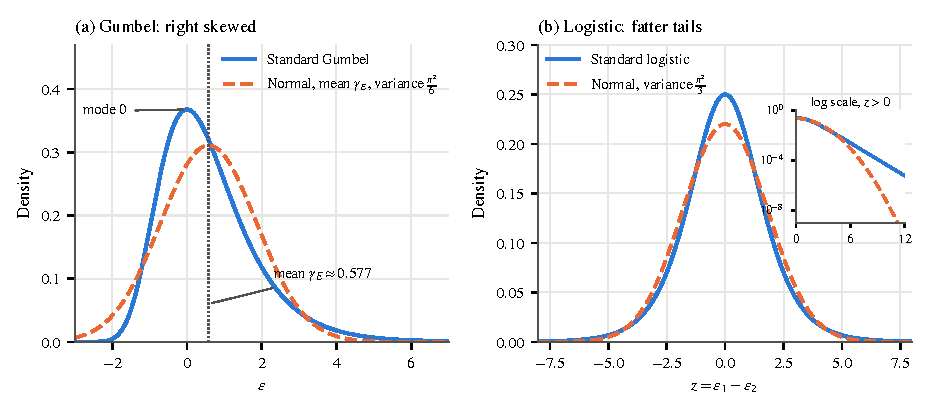
\includegraphics[width=\textwidth]{figures/ch06/gumbel_logistic.pdf}
\caption{Extreme value algebra. (a) The standard Gumbel density (mode $0$, mean $\gamma_E$) against a normal
density with the same mean and variance $\frac{\pi^2}{6}$. (b) The standard logistic density, the distribution of
the difference of two independent standard Gumbels, against a normal density with the same variance
$\frac{\pi^2}{3}$. The inset plots both densities on a log scale for $z > 0$.}
\label{fig:06-gumbel}
\end{figure}

\subsection{Logit choice probabilities}\label{sec:06-logitprob}

\begin{proposition}[Logit choice probabilities]\label{prop:06-logit}
Let $u_{ij} = V_{ij} + \sigma_\epsilon\epsilon_{ij}$ for $j = 0, 1, \dots, J$, with $\epsilon_{ij}$ independent and
identically distributed standard Gumbel and $\sigma_\epsilon > 0$. Then
\begin{equation}\label{eq:06-logit}
P_{ij} = \frac{\exp\left(\frac{V_{ij}}{\sigma_\epsilon}\right)}{\sum_{k=0}^J \exp\left(\frac{V_{ik}}{\sigma_\epsilon}\right)} .
\end{equation}
With $V_{i0} = 0$, $V_{ij} = \delta_j$ for $j \ge 1$ and $\sigma_\epsilon = 1$, the market share is
\begin{equation*}
s_j = \frac{e^{\delta_j}}{1 + \sum_{k=1}^J e^{\delta_k}} .
\end{equation*}
\end{proposition}

\begin{proof}[First proof (direct integration)]
Drop the index $i$ and fix $j$. Product $j$ is chosen when $V_j + \sigma_\epsilon\epsilon_j \ge V_k + \sigma_\epsilon\epsilon_k$
for every $k$, that is, when $\epsilon_k \le \epsilon_j + a_k$ with $a_k = \frac{V_j - V_k}{\sigma_\epsilon}$. Note that
$a_j = 0$. Condition on $\epsilon_j = e$. By independence,
\begin{align*}
P_j &= \int_{-\infty}^{\infty} f(e)\prod_{k\neq j}F(e + a_k)\,\dd e \\
&= \int_{-\infty}^{\infty} e^{-e}\exp\big(-e^{-e}\big)\prod_{k\neq j}\exp\big(-e^{-e}e^{-a_k}\big)\,\dd e \\
&= \int_{-\infty}^{\infty} e^{-e}\exp\Big(-e^{-e}\sum_{k=0}^J e^{-a_k}\Big)\,\dd e ,
\end{align*}
where the factor $\exp(-e^{-e})$ from the density supplies the term $k = j$, since $e^{-a_j} = 1$. Let
$A = \sum_{k=0}^J e^{-a_k} = \sum_{k=0}^J \exp\left(\frac{V_k - V_j}{\sigma_\epsilon}\right)$. Substitute $t = e^{-e}$,
with $\dd t = -e^{-e}\,\dd e$:
\begin{equation*}
P_j = \int_0^\infty e^{-At}\,\dd t = \frac{1}{A}
= \frac{\exp\left(\frac{V_j}{\sigma_\epsilon}\right)}{\sum_{k=0}^J \exp\left(\frac{V_k}{\sigma_\epsilon}\right)} . \qedhere
\end{equation*}
\end{proof}

\begin{proof}[Second proof (max-stability)]
Divide utilities by $\sigma_\epsilon$, which does not change choices (\cref{prop:06-normalization}). Let
$W_k = \frac{V_k}{\sigma_\epsilon}$. By \cref{lem:06-maxstable} applied to the alternatives other than $j$,
\begin{equation*}
\max_{k\neq j}(W_k + \epsilon_k) = L_{-j} + \epsilon^*, \qquad L_{-j} = \ln\sum_{k\neq j}e^{W_k},
\end{equation*}
where $\epsilon^*$ is standard Gumbel and independent of $\epsilon_j$. Product $j$ is chosen when
$W_j + \epsilon_j \ge L_{-j} + \epsilon^*$, that is, when $\epsilon^* - \epsilon_j \le W_j - L_{-j}$. By
\cref{lem:06-logistic},
\begin{equation*}
P_j = \Lambda(W_j - L_{-j}) = \frac{1}{1 + e^{L_{-j} - W_j}} = \frac{e^{W_j}}{e^{W_j} + \sum_{k\neq j}e^{W_k}} ,
\end{equation*}
which is \eqref{eq:06-logit}.
\end{proof}

\casehead{Income, constants and the normalization}
Terms common to all alternatives cancel from \eqref{eq:06-logit}. Consider
\begin{equation*}
u_{ij} = \bar u + \alpha(y_i - p_j) + x_j\beta + \xi_j + \sigma_\epsilon\epsilon_{ij}, \qquad
u_{i0} = \bar u + \alpha y_i + \sigma_\epsilon\epsilon_{i0},
\end{equation*}
with a common constant $\bar u$. The factor $\exp\big(\frac{\bar u + \alpha y_i}{\sigma_\epsilon}\big)$ appears in the
numerator and in every term of the denominator, so it cancels:
\begin{equation*}
P_{ij} = \frac{\exp\left(\frac{x_j\beta + \xi_j - \alpha p_j}{\sigma_\epsilon}\right)}
{1 + \sum_{k=1}^J\exp\left(\frac{x_k\beta + \xi_k - \alpha p_k}{\sigma_\epsilon}\right)} .
\end{equation*}
The probabilities depend on the parameters only through $\frac{\beta}{\sigma_\epsilon}$, $\frac{\alpha}{\sigma_\epsilon}$
and $\frac{\xi_j}{\sigma_\epsilon}$. Only one of the price coefficient and the scale of the shock can be normalized.
The usual choice sets $\sigma_\epsilon = 1$ and estimates $\alpha$, so that
$\delta_j = x_j\beta - \alpha p_j + \xi_j$ is measured in units of the shock. The alternative sets $\alpha = 1$
and estimates $\sigma_\epsilon$, so that utility is measured in dollars and $\sigma_\epsilon$ is the dollar scale of
the taste shocks. Writing $u_{ij} = (y_i - p_j) + \delta_j + \epsilon_{ij}$ with a standard Gumbel shock imposes
both normalizations at once. That specification assumes the standard deviation of the taste shock equals
$\frac{\pi}{\sqrt 6} \approx 1.28$ dollars, a restriction that the data cannot test once the price coefficient is fixed.

\casehead{The two limits of the scale}
Write \eqref{eq:06-logit} as
$P_j = \Big[\sum_k \exp\Big(\frac{V_k - V_j}{\sigma_\epsilon}\Big)\Big]^{-1}$. As $\sigma_\epsilon \to 0$, every term
with $V_k < V_j$ vanishes and every term with $V_k > V_j$ explodes. If $V_j$ is the unique maximum, then
$P_j \to 1$. If some $V_k$ exceeds $V_j$, then $P_j \to 0$. Choice becomes deterministic, and the consumer picks
$\arg\max_k V_k$. As $\sigma_\epsilon \to \infty$, every term tends to one, and $P_j \to \frac{1}{J+1}$. Choice
becomes uniform and ignores the attributes. The scale $\sigma_\epsilon$, or its inverse
$\mu_\epsilon = \frac{1}{\sigma_\epsilon}$, is the bridge to the ``modified BLP'' model of \citet{BerryPakes2007}.
BLP abbreviates the random coefficients logit of Berry, Levinsohn and Pakes \citep{BerryLevinsohnPakes1995}, the
subject of \cref{ch:blp}. The modified BLP model adds $\sigma_\epsilon\epsilon_{ij}$ to a pure characteristics model, and it approaches the pure
characteristics model as $\sigma_\epsilon \to 0$ (\cref{sec:06-epsilon}).

\begin{remark}[The logit as a model of tastes for products]\label{rem:06-tastesforproducts}
\citet[p.~1412]{McFadden1984} observes that the multinomial logit is a special case of a random coefficients
model in which only the coefficients of alternative-specific dummy variables are random. Write
\begin{equation*}
u_{ij} = V_{ij} + \sum_{k=0}^J \epsilon_{ik}\,d_{jk}, \qquad d_{jk} = \indic\{j = k\}.
\end{equation*}
The dummy $d_{jk}$ is a ``characteristic'' that only product $k$ possesses, and $\epsilon_{ik}$ is consumer $i$'s
random taste for it. \citet{BerryPakes2007} attribute this reading to \citet{CaplinNalebuff1991} and call such
models models with ``tastes for products''. Under this reading the dimension of the characteristic space grows
with the number of products. \Cref{sec:06-epsilon} shows that this growth drives the logit's implications for
markups and welfare as products are added.
\end{remark}

\subsection{Expected maximum utility and the log-sum formula}\label{sec:06-logsum}

\begin{proposition}[Log-sum formula]\label{prop:06-logsum}
Under the assumptions of \cref{prop:06-logit},
\begin{equation}\label{eq:06-logsum}
\E\Big[\max_k u_{ik}\Big] = \sigma_\epsilon\ln\sum_{k=0}^J\exp\left(\frac{V_{ik}}{\sigma_\epsilon}\right) + \sigma_\epsilon\gamma_E .
\end{equation}
Its gradient with respect to $(V_{i0}, \dots, V_{iJ})$ is the vector of logit probabilities
\eqref{eq:06-logit}. In addition, the distribution of the maximum utility does not depend on which alternative
attains it: for every $j$ and $x$,
\begin{equation}\label{eq:06-maxindep}
\Pr\Big(j \text{ chosen and } \max_k u_{ik} \le x\Big) = P_{ij}\,\Pr\Big(\max_k u_{ik} \le x\Big).
\end{equation}
\end{proposition}

\begin{proof}
Write $\max_k(V_k + \sigma_\epsilon\epsilon_k) = \sigma_\epsilon\max_k\big(\frac{V_k}{\sigma_\epsilon} + \epsilon_k\big)$. By
\cref{lem:06-maxstable}, $\max_k\big(\frac{V_k}{\sigma_\epsilon} + \epsilon_k\big)$ is Gumbel with location
$\ln\sum_k e^{\frac{V_k}{\sigma_\epsilon}}$ and scale one, so its mean is that location plus $\gamma_E$.
Multiplying by $\sigma_\epsilon$ gives \eqref{eq:06-logsum}. Differentiating,
\begin{equation*}
\frac{\partial}{\partial V_j}\left[\sigma_\epsilon\ln\sum_k e^{\frac{V_k}{\sigma_\epsilon}}\right]
= \sigma_\epsilon\cdot\frac{1}{\sigma_\epsilon}\,\frac{e^{\frac{V_j}{\sigma_\epsilon}}}{\sum_k e^{\frac{V_k}{\sigma_\epsilon}}} = P_j ,
\end{equation*}
as \cref{thm:06-wdz} requires.

For \eqref{eq:06-maxindep}, set $\sigma_\epsilon = 1$ without loss of generality. When $j$ is chosen, the maximum
equals $V_j + \epsilon_j$. Repeating the first proof of \cref{prop:06-logit} with the extra restriction
$V_j + e \le x$,
\begin{align*}
\Pr\Big(j \text{ chosen and } \max_k u_k \le x\Big)
&= \int_{-\infty}^{x - V_j} e^{-e}\exp\big(-Ae^{-e}\big)\,\dd e \\
&= \int_{e^{-(x - V_j)}}^{\infty} e^{-At}\,\dd t \\
&= \frac{1}{A}\exp\big(-Ae^{-(x - V_j)}\big),
\end{align*}
with $A = \sum_k e^{V_k - V_j}$. Since $\frac{1}{A} = P_j$ and $Ae^{V_j} = \sum_k e^{V_k}$, the last expression equals
$P_j\exp\big(-e^{-x}\sum_k e^{V_k}\big)$. By the proof of \cref{lem:06-maxstable} the second factor is
$\Pr(\max_k u_k \le x)$.
\end{proof}

Equation \eqref{eq:06-maxindep} says that the identity of the chosen alternative and the level of the maximum
utility are independent. Consumers who choose a product with low $V_j$ have, on average, a large
$\epsilon_j$ that exactly compensates. All buyers therefore enjoy the same expected utility, whatever they bought.
In the two-goods example of \cref{sec:06-twogoods}, the expected maximum utility is $\ln(1 + e^{0.5} + e) + \gamma_E \approx 2.26$.
A simulation with two million draws gives conditional means of $2.26$ for each of the three choices.

\casehead{Logit consumer surplus}
Combine \eqref{eq:06-logsum} with the welfare formula \eqref{eq:06-smallrosen}. Let
$u_{ij} = \alpha(y_i - p_j) + x_j\beta + \xi_j + \epsilon_{ij}$ for $j \ge 1$ and $u_{i0} = \alpha y_i + \epsilon_{i0}$,
with $\sigma_\epsilon = 1$ and $\delta_j = x_j\beta - \alpha p_j + \xi_j$. Then
$\E[\max_k u_{ik}] = \alpha y_i + \ln\big(1 + \sum_k e^{\delta_k}\big) + \gamma_E$, and dividing by the marginal utility
of income gives the expected consumer surplus
\begin{equation}\label{eq:06-logitcs}
CS_i = \frac{1}{\alpha}\ln\Big(1 + \sum_{k=1}^J e^{\delta_k}\Big) + C ,
\end{equation}
where $C = y_i + \frac{\gamma_E}{\alpha}$ is a constant that drops out of every comparison. For a change from a
choice set $\mathcal{J}^0$ with mean utilities $\delta^0$ to a choice set $\mathcal{J}^1$ with mean utilities $\delta^1$,
\begin{equation}\label{eq:06-logitdcs}
\Delta CS_i = \frac{1}{\alpha}\left[\ln\Big(1 + \sum_{k\in\mathcal{J}^1}e^{\delta^1_k}\Big)
- \ln\Big(1 + \sum_{k\in\mathcal{J}^0}e^{\delta^0_k}\Big)\right].
\end{equation}
Because $1 + \sum_k e^{\delta_k} = \frac{1}{s_0}$ in the logit, \eqref{eq:06-logitcs} can be written
$CS_i = -\frac{1}{\alpha}\ln s_0 + C$, and \eqref{eq:06-logitdcs} becomes
$\Delta CS_i = \frac{1}{\alpha}\ln\frac{s_0^0}{s_0^1}$. In the logit, the outside share and the price coefficient
alone determine the welfare change. In the two-goods example the rise in $\delta_1$ from $0.5$ to $1.3$
lowers $s_0$ from $0.186$ to $0.135$, a gain of $\ln\frac{0.186}{0.135} \approx 0.32$ utils, or
$\frac{0.32}{\alpha}$ dollars. Differentiating \eqref{eq:06-logitcs} with respect to $p_j$ gives
$-\frac{1}{\alpha}\cdot\frac{\alpha e^{\delta_j}}{1 + \sum_k e^{\delta_k}} = -s_j$, the logit version of the Roy
identity noted after \cref{cor:06-wdz}. The logit elasticities and the Berry inversion are in \cref{ch:logit},
and the welfare value of new goods is in \cref{ch:newgoods}. \Cref{sec:06-epsilon} shows that
\eqref{eq:06-logitdcs} assigns positive value to every added product, including an exact copy of an existing one.

\subsection{Luce's axiom, IIA and the generalized extreme value family}\label{sec:06-gev}

\casehead{The choice axiom and IIA}
\citet{Luce1959} proposed an axiom for probabilistic choice. Let $P(j \mid C)$ be the probability of choosing
$j$ from a set $C$. The \emph{choice axiom} requires $P(j \mid C) = P(j \mid A)\,P(A \mid C)$ for every subset
$A \subseteq C$ that contains $j$, where $P(A \mid C) = \sum_{k\in A}P(k \mid C)$. When all probabilities are
positive, the axiom implies that there are scale values $w_k > 0$ with
$P(j \mid C) = \frac{w_j}{\sum_{k \in C} w_k}$. The logit is the case $w_k = e^{V_k}$. The axiom is
equivalent to the \emph{independence of irrelevant alternatives} (IIA): the odds of choosing $j$ over $k$ do not
depend on the other alternatives. In the logit,
\begin{equation}\label{eq:06-iia}
\frac{P_j}{P_k} = \exp\left(\frac{V_j - V_k}{\sigma_\epsilon}\right) ,
\end{equation}
which depends only on $j$ and $k$. \citet[eq.~3.17, p.~1413]{McFadden1984} states the property for a model in
which $V_j = x_j\theta$ depends only on the attributes of $j$: $\ln\frac{P_j}{P_k} = (x_j - x_k)\theta$, independent
of the attributes of every other alternative.

IIA has three consequences. First, the probabilities for a smaller or larger choice set follow from
\eqref{eq:06-logit} by deleting or adding terms in the denominator. A model estimated on existing alternatives
can then forecast the demand for a new one, provided the new alternative brings no new parameters
\citep[p.~1414]{McFadden1984}. Second, the cross-elasticity of the probability of $j$ with respect to an attribute
of $k$ is the same for every $j \neq k$ (p.~1414). A rise in the price of $k$ sends its customers to the other
alternatives in proportion to their shares, as the two-goods example showed. Third, ranked data can be used.
The probability of a complete ranking is the product of logit probabilities of choosing the best alternative
from successively smaller sets \citep{Marschak1960}. \citet[p.~1414]{McFadden1984} calls IIA ``theoretically
implausible in many applications'', while noting that the logit often fits and predicts well in practice.

\begin{remark}[Why Gumbel]\label{rem:06-yellott}
Is the Gumbel distribution the only way to obtain Luce's axiom from random utility? \citet{Yellott1977} studies
random utility models with independent and identically distributed errors from a location family. He shows
that in this class the choice axiom holds for all choice sets of at least three alternatives only if the errors
are Gumbel. We
state the result without proof. It explains why the logit and the independent Gumbel model are the same
object.
\end{remark}

\begin{remark}[Universal logit]\label{rem:06-universal}
IIA comes from restricting $V_j$ to depend on the attributes of $j$ alone. The logistic functional form does
not imply it by itself. Suppose instead that $V_j = z_j(x)\theta$ may depend on the attributes $x$ of all
alternatives. Then the logit form
\begin{equation*}
P_j = \frac{e^{z_j(x)\theta}}{\sum_k e^{z_k(x)\theta}}
\end{equation*}
can approximate any continuous positive response probability model on a compact set, to any desired accuracy
\citep[eq.~3.18, pp.~1414--1415]{McFadden1984}. This \emph{universal logit} can describe any pattern of
cross-elasticities. The approximation may be computationally impractical, and it makes consistency with
utility maximization hard to impose or verify. Its main use is to suggest specification tests (p.~1415).
\end{remark}

The most common test of IIA uses the property that the logit parameters are the same on any subset of the
choice set. Let $\hat\beta_C$ and $\hat V_C$ be the estimates and their estimated covariance matrix from the full
choice set $C$, and $\hat\beta_D$ and $\hat V_D$ those from a subset $D$. Under IIA both estimators are consistent
and the full-set estimator is efficient, so
\begin{equation}\label{eq:06-hmtest}
S = (\hat\beta_D - \hat\beta_C)^\T(\hat V_D - \hat V_C)^{-1}(\hat\beta_D - \hat\beta_C)
\end{equation}
is asymptotically chi-squared with degrees of freedom equal to the rank of $\hat V_D - \hat V_C$
\citep[eq.~3.23, pp.~1417--1418]{McFadden1984}. \citet{HausmanMcFadden1984} analyze the test. McFadden warns
that it is an omnibus test and that it has little power unless the departures from the logit are substantial.
\Cref{ch:logit} applies it.

\begin{remark}[Aggregating alternatives]\label{rem:06-aggregation}
The logit form survives aggregation of alternatives into types \citep[eqs.~3.19--3.20, p.~1415]{McFadden1984}.
Suppose type $g$ contains $M_g$ elemental alternatives with attributes $x_{gj}$ and mean attributes
$\bar x_g$. The probability of choosing some alternative of type $g$ is
\begin{align*}
\sum_{j \in g}P_{gj} &= \frac{\sum_{j \in g}e^{x_{gj}\theta}}{\sum_h\sum_{l \in h}e^{x_{hl}\theta}}, \qquad
\sum_{j\in g}e^{x_{gj}\theta} = \exp\big(\bar x_g\theta + \ln M_g + \omega_g\big),
\end{align*}
where $\omega_g = \ln\Big[\frac{1}{M_g}\sum_{j\in g}e^{(x_{gj} - \bar x_g)\theta}\Big]$ corrects for heterogeneity
within the type and is zero when the alternatives in $g$ are identical. Choice among types is therefore a logit
with utility $\bar x_g\theta + \ln M_g + \omega_g$. The term $\ln M_g$ shows how the logit counts products. Doubling
the number of alternatives of a type, with the new ones identical to the old, adds $\ln 2$ to the utility of
the type. This is the tastes-for-products reading of \cref{rem:06-tastesforproducts} at
work.
\end{remark}

\begin{remark}[Sampling alternatives]\label{rem:06-sampling}
IIA has a practical use when the choice set is large, as when households choose among thousands of houses. The
denominator of each logit probability then sums over every alternative. \citet[sec.~3.6, pp.~1416--1417]{McFadden1984}
shows that the logit can be estimated from a sampled subset of alternatives for each consumer. Let $C$ be the full
choice set, and let consumer $i$ choose $j_i \in C$. The researcher draws a subset $\mathcal{D}_i \subseteq C$ that
contains $j_i$, under a known protocol that selects $\mathcal{D}$ with probability $r(\mathcal{D} \mid j_i, x_i)$. We
write $r$ for McFadden's $\pi$, which this book reserves for profit. The protocol must have the \emph{positive
conditioning property}: $r(\mathcal{D}_i \mid k, x_i) > 0$ for every $k \in \mathcal{D}_i$. Had any member of
$\mathcal{D}_i$ been chosen, the protocol could have produced the same subset.

The probability that consumer $i$ chose $k$, given the sampled subset, follows from Bayes' rule:
\begin{equation*}
\Pr(j_i = k \mid \mathcal{D}_i, x_i)
= \frac{P_k(x_i, \theta)\, r(\mathcal{D}_i \mid k, x_i)}{\sum_{l \in \mathcal{D}_i} P_l(x_i, \theta)\, r(\mathcal{D}_i \mid l, x_i)} .
\end{equation*}
The sum runs over $\mathcal{D}_i$ only, because the protocol never produces a subset that excludes the chosen
alternative. We substitute the logit $P_k(x_i, \theta) = \frac{e^{x_{ik}\theta}}{\sum_{m \in C}e^{x_{im}\theta}}$. The
full-set denominator appears in every term and cancels, which leaves
\begin{equation}\label{eq:06-sampled-logit}
\Pr(j_i = k \mid \mathcal{D}_i, x_i)
= \frac{\exp\big(x_{ik}\theta + \ln r(\mathcal{D}_i \mid k, x_i)\big)}{\sum_{l \in \mathcal{D}_i}\exp\big(x_{il}\theta + \ln r(\mathcal{D}_i \mid l, x_i)\big)} .
\end{equation}
This is a logit on $\mathcal{D}_i$ with $\ln r(\mathcal{D}_i \mid k, x_i)$ added to each utility. Positive conditioning
keeps every logarithm finite. The average of $\ln\Pr(j_i \mid \mathcal{D}_i, x_i)$ over consumers is McFadden's modified
log-likelihood (his eq.~3.22). Under positive conditioning and a standard identification condition, its maximizer is
consistent for $\theta$. It is a conditional likelihood, so the inverse of its information matrix estimates the
covariance matrix as usual (p.~1417).

The correction cancels when $r(\mathcal{D}_i \mid k, x_i)$ is the same for every $k \in \mathcal{D}_i$, the
\emph{uniform conditioning property}. McFadden's example draws the chosen alternative and one other alternative at
random (his eq.~3.21):
\begin{equation*}
r(\mathcal{D} \mid j_i, x_i) = \begin{cases} \frac{1}{|C| - 1} & \text{if } \mathcal{D} = \{j_i, k\} \text{ with } k \neq j_i,\\
0 & \text{otherwise,}\end{cases}
\end{equation*}
where $|C|$ is the number of alternatives. Either member of $\mathcal{D}_i$, had it been chosen, would have produced
$\mathcal{D}_i$ with the same probability. The logit can then be estimated from binary choices between the chosen
alternative and one random rival. The argument needs IIA. The full-set denominator cancels only because the ratio
$\frac{P_k}{P_l}$ does not depend on the alternatives outside $\mathcal{D}_i$.
\end{remark}

\casehead{Generalized extreme value models}
\citet{McFadden1978} found a class of joint distributions for the shocks that keeps closed forms while
relaxing IIA. Models in this class are called \emph{generalized extreme value} (GEV) models.

\begin{theorem}[Generalized extreme value models]\label{thm:06-gev}
Let $H : \R^{J+1}_+ \to \R_+$ satisfy three conditions.
\begin{enumerate}[label=(G\arabic*)]
  \item $H$ is homogeneous of degree one: $H(\lambda y) = \lambda H(y)$ for $\lambda > 0$.
  \item $H(y) \to \infty$ as $y_j \to \infty$, for any $j$.
  \item For any $r$ distinct indices $j_1, \dots, j_r$, the mixed partial derivative
  $\frac{\partial^r H}{\partial y_{j_1}\cdots\partial y_{j_r}}$ is nonnegative if $r$ is odd and nonpositive if $r$
  is even.
\end{enumerate}
Then the following hold.
\begin{enumerate}[label=(\alph*)]
  \item $F(\epsilon_0, \dots, \epsilon_J) = \exp\big(-H(e^{-\epsilon_0}, \dots, e^{-\epsilon_J})\big)$ is the CDF of a
  multivariate extreme value distribution whose marginals are Gumbel.
  \item In the ARUM $u_j = V_j + \epsilon_j$ with $\epsilon$ distributed as in (a), the choice probabilities are
  \begin{equation}\label{eq:06-gevprob}
  P_j = \frac{y_j H_j(y)}{H(y)} = \frac{\partial\ln H(e^{V_0}, \dots, e^{V_J})}{\partial V_j},
  \qquad y = (e^{V_0}, \dots, e^{V_J}),
  \end{equation}
  where $H_j$ is the partial derivative of $H$ with respect to its $j$-th argument.
  \item The social surplus function is $G(V) = \ln H(e^{V_0}, \dots, e^{V_J}) + \gamma_E$.
\end{enumerate}
\end{theorem}

\begin{proof}
Part (a) is the theorem of \citet{McFadden1978}, restated by \citet[eqs.~3.29--3.31, p.~1421]{McFadden1984}.
We take it as given. Its marginals follow by sending the other arguments to infinity:
$F_j(\epsilon_j) = \exp\big(-e^{-\epsilon_j}H(e_j)\big)$, a Gumbel CDF with location $\ln H(e_j)$, where $e_j$ is the
$j$-th unit vector.

For (c), the maximum is at most $x$ if and only if $\epsilon_k \le x - V_k$ for every $k$. Using (a) and then
homogeneity with $\lambda = e^{-x}$,
\begin{equation*}
\Pr\Big(\max_k(V_k + \epsilon_k) \le x\Big) = \exp\Big(-H\big(e^{V_0 - x}, \dots, e^{V_J - x}\big)\Big)
= \exp\Big(-e^{-\left(x - \ln H(y)\right)}\Big).
\end{equation*}
The maximum is Gumbel with location $\ln H(y)$, so its mean is $\ln H(y) + \gamma_E$.

For (b), the density of the event that $j$ is chosen with $\epsilon_j = e$ is $\frac{\partial F}{\partial\epsilon_j}$
evaluated at $\epsilon_k = e + V_j - V_k$ for all $k$. Differentiating $F$,
\begin{equation*}
\frac{\partial F}{\partial \epsilon_j}(\epsilon) = F(\epsilon)\,H_j(e^{-\epsilon_0}, \dots, e^{-\epsilon_J})\,e^{-\epsilon_j}.
\end{equation*}
At the evaluation point, $e^{-\epsilon_k} = \lambda y_k$ with $\lambda = e^{-e - V_j} = \frac{e^{-e}}{y_j}$. Homogeneity of
degree one implies $H(\lambda y) = \lambda H(y)$, and its derivative $H_j$ is homogeneous of degree zero, so
$H_j(\lambda y) = H_j(y)$. Hence
\begin{align*}
P_j &= \int_{-\infty}^{\infty}\exp\Big(-\frac{e^{-e}}{y_j}H(y)\Big)H_j(y)\,e^{-e}\,\dd e \\
&= H_j(y)\int_0^\infty\exp\Big(-t\,\frac{H(y)}{y_j}\Big)\,\dd t
= \frac{y_jH_j(y)}{H(y)},
\end{align*}
where the second line substitutes $t = e^{-e}$. Finally,
$\frac{\partial\ln H(e^{V})}{\partial V_j} = \frac{H_j(y)\,e^{V_j}}{H(y)}$, which is the same expression. It equals the
derivative of $G$ in (c), as \cref{thm:06-wdz} requires.
\end{proof}

The logit is the generating function $H(y) = \sum_j y_j$. It satisfies (G1) and (G2), its first derivatives
equal one, and its higher mixed derivatives vanish. Then $F(\epsilon) = \prod_j\exp(-e^{-\epsilon_j})$, the shocks
are independent, and \eqref{eq:06-gevprob} gives $P_j = \frac{y_j}{\sum_k y_k}$. McFadden's version,
$H(y) = \big(\sum_j y_j^{\frac{1}{\lambda}}\big)^{\lambda}$ with $0 < \lambda \le 1$, gives the logit with scale $\lambda$
\citep[eq.~3.32, p.~1421]{McFadden1984}.

The nested logit is the leading member of the family that relaxes IIA. Partition the inside products into nests
$g = 1, \dots, G$, and place the outside good in its own nest. With nesting parameter $\sigma \in [0, 1)$, let
\begin{equation}\label{eq:06-nestedH}
H(y) = y_0 + \sum_{g=1}^G\Big(\sum_{j\in g}y_j^{\frac{1}{1-\sigma}}\Big)^{1-\sigma}.
\end{equation}
Write $D_g = \sum_{k\in g}y_k^{\frac{1}{1-\sigma}}$. For $j$ in nest $g$, the derivative is
$H_j = D_g^{-\sigma}\,y_j^{\frac{\sigma}{1-\sigma}}$, so $y_jH_j = D_g^{-\sigma}y_j^{\frac{1}{1-\sigma}}$ and
\begin{equation*}
P_j = \frac{y_j^{\frac{1}{1-\sigma}}}{D_g}\cdot\frac{D_g^{1-\sigma}}{y_0 + \sum_{h=1}^G D_h^{1-\sigma}} .
\end{equation*}
The first factor is the probability of choosing $j$ within its nest, and the second is the probability of
choosing nest $g$. With $\sigma = 0$ the model is the logit. As $\sigma$ approaches one, the products within a
nest become close substitutes. \citet[sec.~3.10, pp.~1422--1425]{McFadden1984} develops the general
hierarchical version, the nested multinomial logit, with an ``independence'' parameter at each node, here
$1 - \sigma$. He notes that estimates of these parameters outside the unit interval indicate a misspecified tree
(pp.~1425--1426), and that the likelihood is not concave in all parameters (p.~1426). \Cref{ch:logit} develops
the nested logit, its elasticities and its estimation.

\subsection{The multinomial probit}\label{sec:06-probit}

The \emph{multinomial probit} assumes jointly normal shocks, $\epsilon_i \sim N(0, \Sigma_\epsilon)$, with a
$(J+1)\times(J+1)$ covariance matrix $\Sigma_\epsilon$. Product $j$ is chosen when
$\epsilon_{ik} - \epsilon_{ij} \le V_{ij} - V_{ik}$ for every $k \neq j$. The vector of these $J$ differences is
normal with covariance matrix $B_j\Sigma_\epsilon B_j^\T$, where $B_j$ is the $J\times(J+1)$ matrix that
subtracts $\epsilon_{ij}$ from the other shocks. The choice probability is a $J$-dimensional normal orthant
probability, which has no closed form \citep[sec.~3.8]{McFadden1984}. A version with an economic
interpretation sets $u_{ij} = x_{ij}a_i$ with normally distributed taste weights $a_i \sim N(\beta, \Omega_a)$, so
that utilities have covariance $x_i\Omega_a x_i^\T$ across alternatives (p.~1418).

The probit has the flexibility that the logit lacks. With correlated shocks it does not have IIA, and it
permits very general patterns of cross-elasticities (p.~1418). The cost is computation. McFadden reports that
probabilities with up to three alternatives cost about as much to compute as logit probabilities (p.~1418).
With five or more alternatives and an unrestricted covariance matrix, they were usually too costly for iterative
estimation at the time. The probit log-likelihood is also not known to be concave (p.~1419). One remedy restricts the
covariance with a factor structure,
\begin{equation*}
\epsilon_{ij} = \zeta_{ij} + \sum_{l=1}^{L}\gamma_{jl}v_{il},
\end{equation*}
with independent normal $\zeta_{ij}$ and $v_{il}$ \citep[eq.~3.25, p.~1419]{McFadden1984}. The loading $\gamma_{jl}$ can
be read as the level in alternative $j$ of an unobserved characteristic $l$, and $v_{il}$ as the consumer's random
taste for it. This is a random coefficients model on unobserved characteristics. Simulation methods developed
since then make probit models with many alternatives feasible \citep{Train2009}.

The independent probit, with $\Sigma_\epsilon$ the identity matrix, has essentially the same restrictions on
substitution as the logit, and \citet[p.~1420]{McFadden1984} sees little reason to prefer one over the other.
The lesson matters for the rest of the book. The logit's substitution problems come from shocks that are
independent across products, which leave products with no notion of similarity. The shape of the Gumbel
distribution plays little role. Fixing the problems requires correlation in tastes across similar products. Nesting supplies it within
groups (\cref{ch:logit}), and random coefficients on characteristics supply it along each characteristic
(\cref{ch:blp}).

\subsection{Choosing a functional form}\label{sec:06-forms}

\citet[sec.~3.3]{McFadden1984} judges functional forms by computational practicality and by flexibility in
representing similarity across alternatives. He groups the concrete forms into three families. Logit models
descend from \citet{Luce1959}. Probit models descend from \citet{Thurstone1927}. Elimination models, in which
alternatives are screened out until one remains, descend from \citet{Tversky1972}. His verdict (p.~1410) is that
the multinomial logit scores well on simplicity and computation but poorly on flexibility. The multinomial
probit is simple and flexible but scores poorly on computation. The nested logit and the factor-structure probit
try to achieve both. He adds that functional forms allowing similar substitution patterns tend to fit existing
data comparably. This observation anticipates the strategy of modern empirical work. The choice of a model is
mainly a choice of substitution patterns, and the distribution of the idiosyncratic shock matters mostly through
its implications for computation and welfare.

\begin{remark}[A representative-consumer foundation]\label{rem:06-representative}
Logit demand also arises from a single representative consumer \citep{AndersonDePalmaThisse1988,AndersonDePalmaThisse1992}.
Suppose the consumer allocates one unit of consumption across the alternatives $j = 0, 1, \dots, J$ to maximize
\begin{equation*}
\sum_{j=0}^J \delta_j q_j - \sum_{j=0}^J q_j\ln q_j \qquad \text{subject to} \qquad \sum_{j=0}^J q_j = 1,
\end{equation*}
with $\delta_0 = 0$. The entropy term rewards spreading consumption across products. The first-order conditions
$\delta_j - \ln q_j - 1 - \lambda = 0$, with multiplier $\lambda$, give $q_j \propto e^{\delta_j}$, and the constraint
yields $q_j = \frac{e^{\delta_j}}{1 + \sum_{k\ge 1}e^{\delta_k}}$, the logit shares. A weight $\sigma_\epsilon$ on the entropy
term produces the logit with scale $\sigma_\epsilon$. The two foundations, a population of consumers with Gumbel
shocks and a representative consumer with a taste for variety, give the same aggregate demand.
\Cref{ch:diffprod} gives the full derivation and shows that the constant elasticity of substitution (CES) demand system is a logit in log prices.
\end{remark}
